\documentclass[11pt]{amsart}
\usepackage[demo]{graphicx}
\usepackage{subfigure}

\usepackage[dutch]{babel}
\usepackage{a4wide}
%\setlength{\parindent}{0pt}

\newtheorem*{vraag}{Vraag}
\newtheorem*{uitwerking}{Uitwerking}
\newtheorem*{algoritme}{Algoritme}

\newcommand{\R}{\mathbb{R}}
\newcommand{\N}{\mathbb{N}}
\newcommand{\Z}{\mathbb{Z}}
\newcommand{\C}{\mathbb{C}}
\newcommand{\A}{\mathbb{A}}
\newcommand{\Q}{\mathbb{Q}}
\newcommand{\F}{\mathbb{F}}
\newcommand{\f}{\varphi}
\newcommand{\e}{\varepsilon}
\renewcommand{\d}{\delta}

\begin{document}

\section{Intro}
Het grote nadeel van de Fouriertransformatie is dat een enkele discontinu\"iteit grote gevolgen heeft voor de mate van afname van de co\"effici\"enten. Dit betekent dat compressie in deze gevallen moeilijk wordt. De Waveletbasis is wat anders: elke basisfunctie heeft een compacte drager. Zie de figuur.
\begin{figure}[h]
\subfigure[Impressie van een aantal Fourierbasiselementen]{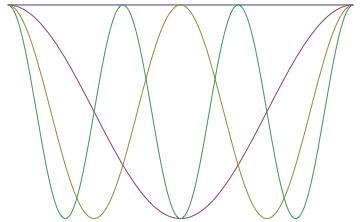
\includegraphics[width=.4\linewidth]{Fourier_basis.jpg}}
\subfigure[Een aantal Morlet-Wavelet basiselementen]{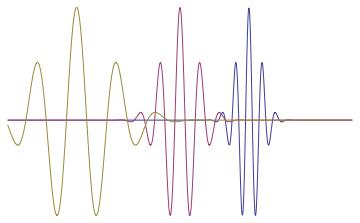
\includegraphics[width=.4\linewidth]{Wavelet_basis.jpg}}
\end{figure}

Het gevolg is dat bij Wavelets discontinu\"iteiten in slechts een deel van de basisfuncties `zichtbaar' zijn. De co\"effici\"enten van de andere basisfuncties nemen op deze manier nog steeds netjes af.

Vanaf nu zullen we (voor het continue geval) aannemen dat een functie/signaal in $L_2$ leeft. Dit is een Hilbertruimte. Laat $\Psi$ een orthonormale basis voor deze ruimte. Als nu een functie $f$ in deze ruimte geschreven wordt in $\Psi$:
\[
f = \sum_{\lambda} \langle f, \psi_\lambda \rangle \psi_\lambda,
\]
dan geldt
\[
||f||^2 = \sum_{\lambda} | \langle f, \psi_\lambda \rangle |^2,
\]
omdat
\[
||f||^2 = \langle f, f \rangle = \left\langle \sum_{\lambda} \langle f, \psi_\lambda \rangle \psi_\lambda, \sum_{\mu} \langle f, \psi_\mu \rangle \psi_\mu \right\rangle = \sum_{\lambda} \sum_{\mu} \left\langle \langle f, \psi_\lambda \rangle \psi_\lambda, \langle f, \psi_\mu \rangle \psi_\mu \right \rangle
\]
\[
 = \sum_\lambda \sum_\mu \langle f, \psi_\lambda \rangle \overline{\langle f, \psi_\mu \rangle}\langle \psi_\lambda, \psi_\mu \rangle = \sum_\lambda \sum_\mu \langle f, \psi_\lambda \rangle \overline{\langle f, \psi_\mu \rangle} \delta_{\lambda \mu} = \sum_\lambda \langle f, \psi_\lambda \rangle \overline{\langle f, \psi_\lambda \rangle} = \sum_\lambda |\langle f, \psi_\lambda \rangle |^2.
\]

Vanaf nu zullen we aannemen dat elke functie in $L_2$ leeft, dus dat $\int |f(x)|^2 dx$ begrensd is. Verder noemen we de gehele ruimte $\Omega$.

Een wavelet geeft aanleiding tot een verzameling basisfuncties met een aantal eigenschappen. De eerste eigenschap is dat ze samen een orthogonale basis
\[
\{ \psi_\lambda: \lambda = (l,j)\text{ met } l \in \N,j \in \Z \}\]
 vormen. Dit betekent dat 
\[
\langle \psi_{\lambda_1}, \psi_{\lambda_2} \rangle = \delta_{\lambda_1, \lambda_2}
\]
 waarbij 
\[
\langle f, g\rangle = \underset{\Omega}{\int} f(x) \overline{g(x)} dx,
\]
met $\overline{g(x)}$ de complex geconjugeerde van $g(x)$.

De tweede eigenschap hebben we al genoemd en is dat deze basisfuncties een compacte drager $S_\lambda$ hebben. Deze basisfuncties worden vaak opgeschreven als $\psi_\lambda = \psi_{l,j}$. De $l$ geeft hierbij de schaling aan en $j$ de verschuiving. Gegeven een Waveletfunctie $\psi$ kunnen we de basisfunctie $\psi_\lambda$ maken door:
\[
	\psi_\lambda(x) = 2^{j/2} \psi(2^jx - k).
\]

Naast deze twee eigenschappen heeft elke wavelet een zogenaamde orde. Wanneer de waveletfunctie loodrecht staat $\langle \psi, q\rangle = 0$ op alle polynomen van graad $p-1$ of lager, spreken we van een wavelet van orde $p$.\footnote{Veel wavelets worden ontworpen met de wil om de orde zo groot mogelijk te maken. Daubechies, Coiflets en Symlets zijn alle drie voorbeelden hiervan.} Dit komt overeen met te zeggen dat
\[
	\int_{-\infty}^\infty x^k \psi(x) dx = 0 \text{ voor } k \in \{ 0, \ldots p-1 \}.
\]

Gevolg van deze eigenschap is dat we $|\langle f, \psi_\lambda\rangle |$ als volgt om kunnen schrijven:
\[
	|\langle f, \psi_\lambda \rangle | = |\langle f-q, \psi_\lambda \rangle | \text{ voor elk polynoom $q$ van graad $p-1$ of lager,} 
\]
zodat
\[
	|\langle f-q, \psi_\lambda \rangle | \leq ||f-q||_\Omega \cdot ||\psi_\lambda||_\Omega.
\]


De continue Wavelettransformatie van een signaal $f(x)$ wordt nu als volgt:
\[
	F(\lambda) = \underset{\Omega}{\int} f(x) \overline{\psi_\lambda(x)} dx = \langle f, \psi_\lambda \rangle.
\]

\subsection{Discrete geval}
Omdat wij het discrete geval bekijken, zullen we kijken naar signalen die als $n$-dimensionale rij $f[k_1,\ldots,k_n]$ geschreven kunnen worden. Daarnaast stellen we voor het gemak dat $k_i$ een tweemacht is die voor elke $i$ hetzelfde is.\footnote{Het geval waarin dit niet zo is is speciaal. Over het algemeen wordt het signaal dan met specifieke waardes aangevuld. Wij gaan hier niet verder op in.} Zo krijgen we dus een $n$-dimensionale ruimte van `roosterpunten'.

TODO: something something filters.

Discreet gaat dit algoritme een stukje anders. We zullen het eendimensionale algoritme uitleggen en aan de hand daarvan in het vervolg het meerdimensionale geval uitwerken.

\begin{algoritme}[Fast Wavelet Transform]
Laat $x[n]$ een signaal van lengte $l = 2^k$. Verder zijn de filters $g[n], h[n],g^*[n], h^*[n]$ gegeven. E\'en niveau van de transformatie gaat nu als volgt.

\begin{quote}
Maak twee nieuwe signalen 
\[
y_l^*[n] = (x * g)[n] = \sum_{k=-\infty}^\infty x[k]g[n-k]
\]
\[
y_h^*[n] = (x * h)[n] = \sum_{k=-\infty}^\infty x[k]h[n-k]
\]
door het oorspronkelijke signaal te colvolueren met beide filters. Vervolgens wordt er ge\emph{subsampled} met een factor twee:
\[
y_l[n] = y_l^*[2n]
\]
\[
y_h[n] = y_h^*[2n].
\]
De rij $y_h$ heet nu de \emph{detail}rij, en $y_l$ de \emph{approximatie}rij.
\end{quote}
Het volgende niveau wordt uitgevoerd met de rij $y_l$ (dus met de helft van de lengte waar we mee begonnen). Dit kan worden herhaald tot de lengte van de approximatierij 1 is. In een plaatje:
\begin{figure}[h]
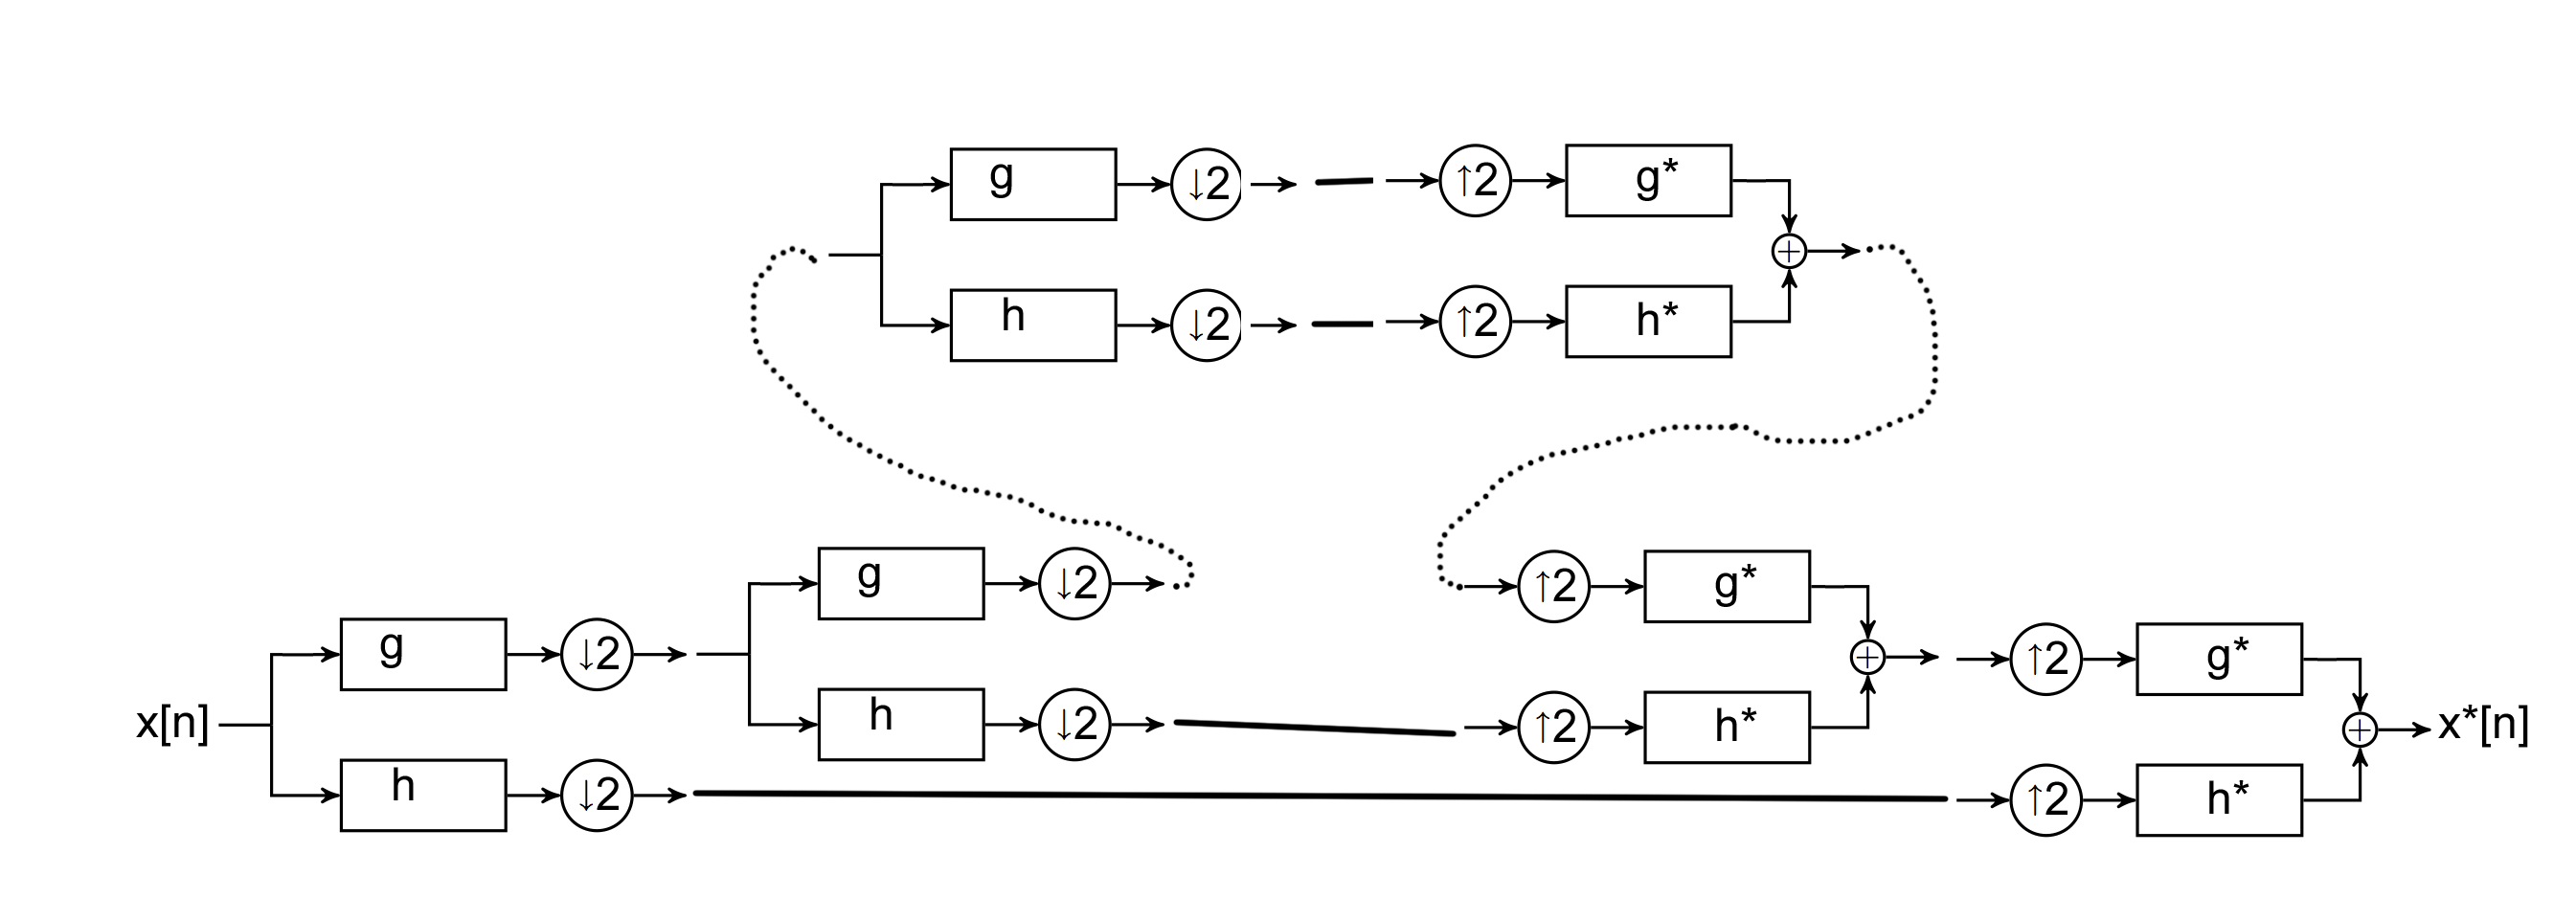
\includegraphics{filter_bank_kankerzuur.jpg}
\end{figure}

Hiermee wordt ook direct het inverse algoritme duidelijk. Gegeven een verzameling rijen $\{y_h, y_{lh}, y_{llh}, \ldots, y_{l^nh}, y_{l^nl}\}$ kunnen we in elke stap het originele signaal $x[n]$ terugvinden door, gegeven de $y_l, y_h$ van die stap:
\[
	y^*_{l}[n] = \begin{cases} y_{l}[n/2] \text{ als } n \mod{2} \equiv 0 \\ 0 \text{ anders}; \end{cases}
\]
\[
	y^*_{h}[n] = \begin{cases} y_{h}[n/2] \text{ als } n \mod{2} \equiv 0 \\ 0 \text{ anders}. \end{cases}
\]
\[
	x[n] = \sum_{k=-\infty}^\infty y^*_{l}[k]g^*[n-k] + \sum_{k=-\infty}^\infty y^*_{h}[k]h^*[n-k]
\]

\end{algoritme}

discontinuiteiten -> matplotlib.

Filter

\section{Discrete Wavelet Transformation en Fast}
Recursief toepassen (plaatje), approximation \& detail coeffs.

\section{Compression}
plaatje met matplotlib

\section{In meer dimensies}

\subsection{Mallat versus Tensor}
Plaatje

\section{Results}
Terminology: PSNR, implementatie (snippets)

\subsection{pt 1: plaatjes}
\subsection{pt 2: filmpjes}

-----

\section{discussion}

BRONNEN

\end{document}
